\documentclass[slovak]{beamer}

\usepackage[slovak]{babel}
\usepackage[utf8]{inputenc}
\usepackage{hyperref}

\usetheme{Madrid}

\title{Konečné automaty}

\author{Matúš Škuta}

\institute[Vysoké učení technické]
{
  Vysoké učení technické v Brne
}
\date{27 apríl 2018}


\begin{document}

\begin{frame}
  \titlepage
\end{frame}

%obsah
\begin{frame}{Obsah}
  \tableofcontents
\end{frame}

\section{Definícia}
\frame
{
    \frametitle{Definícia}
    \bigskip
    Konečný automat z anglického slova "Finite state machine" je výpočetný model primitívneho počítača, ktorý sa skladá z niekoľko stavov a z niekoľko prechodov a ktorý dokáže príjmuť alebo zamietnuť vložené slovo.
    \begin{center}
    \scalebox{0.5}{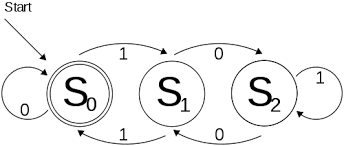
\includegraphics{kon_automat.eps}}
    \end{center}
}


\section{Deterministický konečný automat}
\frame
{
    \frametitle{Deterministický konečný automat}
    Deterministický konečný automat alebo DKA je pätica ($\sum$,$K$,$q_0$,$\delta$,$F$) kde:
    \begin{itemize}
        \item $\sum$ je vstupná abeceda (neprázdna konečná množina symbolov),
        \item $K$ je konečná množina stavov,
        \item $q_0$ je počiatočný stav, pričom platí $q_0 \in K$,
        \item $\delta$ je prechodová funkcia $\delta : K \rightarrow K$, čiže funkcia, ktorá na základe stavu a symbolu zo vstupnej abecedy vráti nový stav,
        \item $F$  je množina akceptačných stavov, je to ľubovoľná (môže byť aj prázdna) podmnožina  $K$.Hovoríme, že DKA akceptuje slovo $\omega$, ak výpočet na tomto slove skončí v niektorom z akceptačných stavov.
    \end{itemize}
}

\section{Konfigurácia a výpočet DKA}
\frame
{
    \frametitle{Konfigurácia a výpočet DKA}
    \begin{block}{Konfigurácia}
        Konfigurácia deterministického konečného automatu je dvojica $(q,\omega) \in K \times \sum^*$ kde $q$ je aktuálny stav automatu a $\omega$ je dosiaľ neprečítaná časť vstupného slova.
    \end{block}
        \begin{block}{Výpočet}
    Krok výpočtu deterministického konečného automatu je relácia $\vdash_A$ na konfiguráciach DKA definovaná nasledovne: $(q,av) \vdash_A(p,v) \Leftrightarrow p = \delta(q,a)$.
    
    Pod výpočtom na deterministickom konečnom automate rozumieme ľubovoľnú postupnosť na seba nadväzujúcich výpočtových krokov.
    \end{block}
}

\section{Nedeterministický konečný automat}
\frame
{
    \frametitle{Nedeterministický konečný automat}
        Nedeterministický konečný automat alebo NKA je pätica ($\sum$,$K$,$q_0$,$\delta$,$F$) kde:
        \begin{itemize}
        \item $\sum$ je vstupná abeceda (neprázdna konečná množina symbolov),
        \item $K$ je konečná množina stavov,
        \item $q_0$ je počiatočný stav, pričom platí $q_0 \in K$,
        \item $\delta$ je prechodová funkcia $\delta : K \times (\sum \cup {e}) \rightarrow 2^K$, čiže funkcia, ktorá na základe stavu a symbolu zo vstupnej abecedy vráti množinu nových stavov,
        \item $F$  je množina akceptačných stavov, je to ľubovoľná (môže byť aj prázdna) podmnožina  $K$.Hovoríme, že NKA akceptuje slovo $\omega$, ak výpočet na tomto slove skončí v niektorom z akceptačných stavov.
    \end{itemize}
}

\section{Konfigurácia a výpočet NKA}
\frame
{
    \frametitle{Konfigurácia a výpočet NKA}
    \begin{block}{Konfigurácia}
        Konfigurácia nedeterministického konečného automatu sa definuje analogicky, ako pri deterministických konečných automatoch. Je to dvojica $(q,\omega) \in K \times \sum^*$ kde $q$ je aktuálny stav automatu a $\omega$ je dosiaľ neprečítaná časť vstupného slova.
    \end{block}
        \begin{block}{Výpočet}
    Krok výpočtu deterministického konečného automatu je relácia $\vdash_A$ na konfiguráciach NKA $A$ definovaná nasledovne: $(q,aw) \vdash_A(p,w) \Leftrightarrow p = \delta(p,a)$.
    \end{block}
}

\section{Ekvivalencia a rozdiely medzi DKA a NKA}
\frame
{
    \frametitle{Ekvivalencia a rozdiely medzi DKA a NKA}
    \begin{block}{Ekvivalencia}
    V skutočnosti, napriek rozdielnej definícii oboch výpočtových modelov, je ich výpočtová sila rovnaká. Je dokázané, že ku každému nedeterministickému automatu $A$ existuje deterministický konečný automat $B$ taký, že $L(B) = L(A)$. Opačná inklúzia je zrejmá z faktu, že deterministický automat je špeciálny prípad nedeterministického.
    \end{block}
    \begin{block}{Rozdiely}
    Existujú teda dva podstatné rozdiely medzi NKA a DKA:
    \begin{itemize}
        \item NKA povoľujú prechody na $\varepsilon$
        \item Nový stav nie je pre každý prechod určený jednoznačne. Prechodová funkcia vracia celú množinu stavov (pri výpočte sa môže postupovať do ľubovoľného z nich), ktorá môže byť dokonca prázdna.
    \end{itemize}
    \end{block}
}

\begin{frame}{Zdroje}
\begin{itemize}
\item \url{https://matematika.cz/konecny-automat}
\item \url{https://sk.wikipedia.org/wiki/Kone\%C4\%8Dn\%C3\%BD_automat}
\end{itemize}

\end{frame}

\end{document}
